\subsection{Conociendo el estado actual}

Con la notación de las arquitecturas objetivo establecidas, al igual que el desarrollo del módulo encargado de la construcción y validación de los archivos de configuración; lo siguiente era la definición del proceso de la comparación entre la arquitectura actual y la arquitectura de referencia. Este proceso, permitirá evaluar el estado del sistema y, por consiguiente, establecer las acciones a tomar con el fin de adaptar la arquitectura hacia el estado objetivo establecido.

Esto requiere conocer el estado actual del sistema, al igual que el conocer el estado objetivo. Siendo así, y ya teniendo la posibilidad de declarar las necesidades de la aplicación, lo siguiente es establecer una manera de determinar el estado del sistema. Dado el enfoque hacia los datos recolectados, es necesario el precisar la manera en la que conoceríamos en qué estado se encuentra el sistema.

Lo primero era el identificar los puntos de acceso por los cuales podríamos acceder a los datos. En el caso de Smart Campus UIS, y teniendo en cuenta que el modelo que se definió depende de los mensajes enviados por los dispositivos, como se observa en la figura \ref{fig:ArquitecturaSmartCampus}, existen dos opciones para procesar estos mensajes. 

La primera, es consultar los mensajes enviados usando uno de los endpoints del servicio \texttt{data\_microservice}, lo que da acceso a todos los mensajes registrados. Y, la segunda, usando el mismo bus de datos, empleado por los servicios de la plataforma, lo que permitiría el acceso, incluso de manera más directa, a los mensajes a medida que estos son enviados.

\begin{figure}[ht]
    \centering
    \caption{\\Arquitectura del prototipo de Smart Campus definido por }\citeA{msc_henry_2022}
    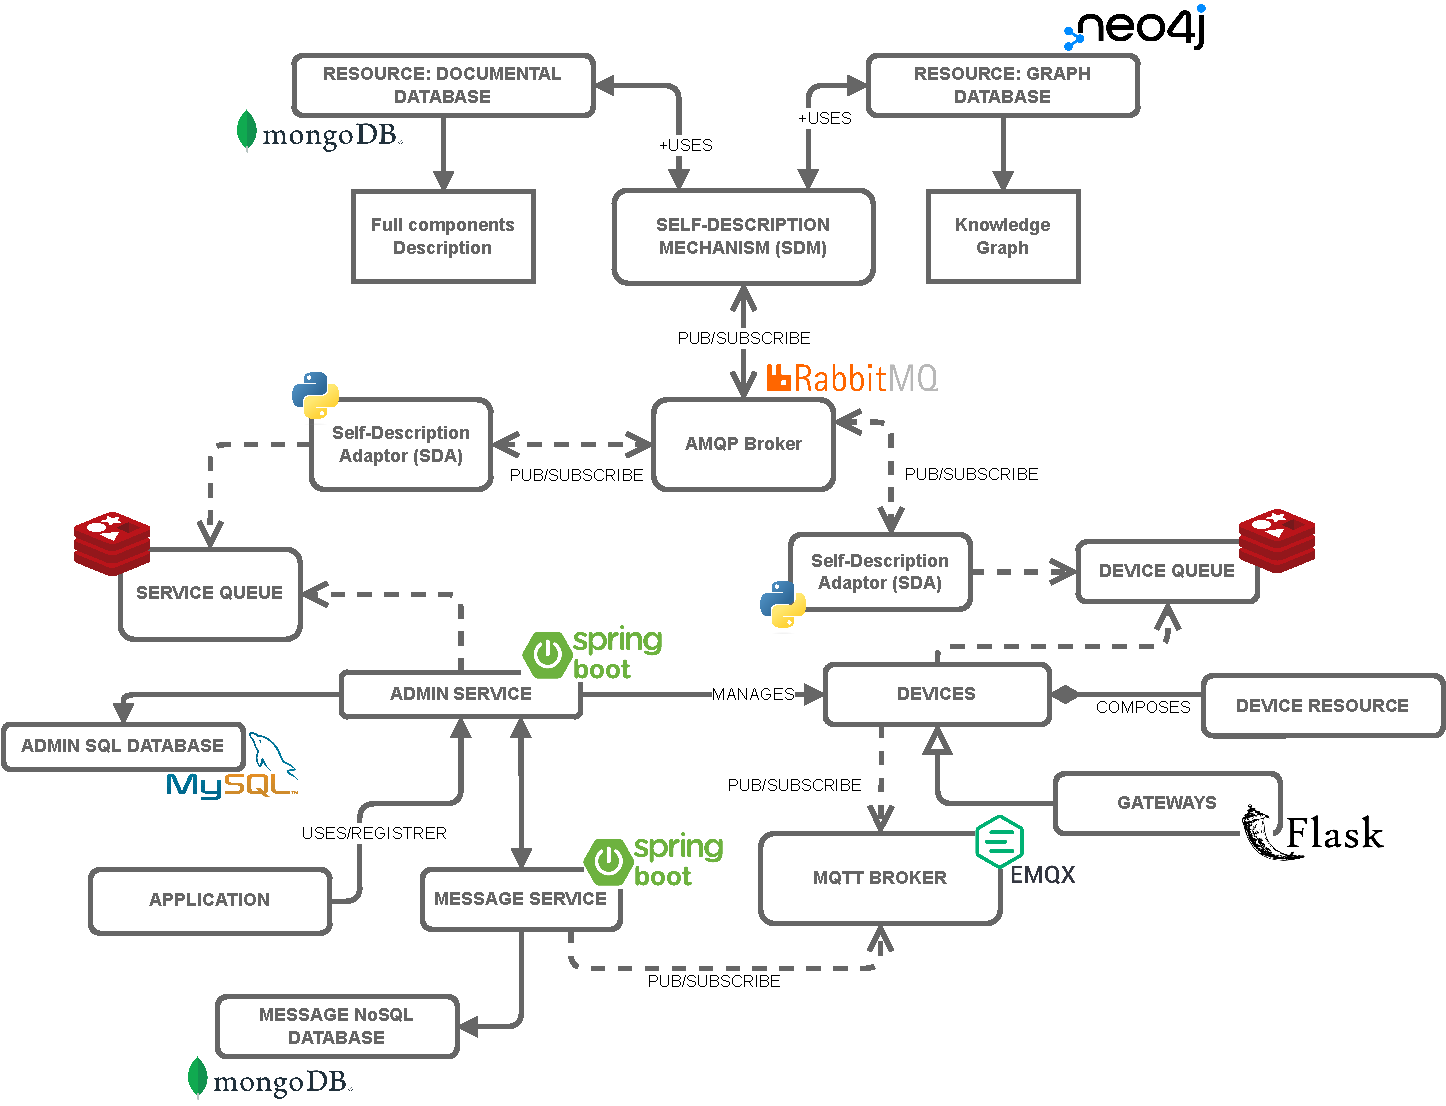
\includegraphics[width=\linewidth]{images/ArquitecturaSmartCampusUis.pdf}
    \label{fig:ArquitecturaSmartCampus}
\end{figure}

Ahora, cada una de las maneras de acceder a los datos es viable, y podría permitir la implementación correspondiente para determinar el estado del sistema. Sin embargo, de entre las dos opciones, se escogió el procesamiento de los mensajes enviados por los dispositivos, enviados por MQTT. 

Esto se debe a varios factores, principalmente, debido a cómo se consultan los mensajes desde el endpoint. Para realizar esta consulta, es necesario conocer el \textit{UUID} del dispositivo a consultar lo que, como se evidenció durante la validación de los requerimientos de datos en la sección \ref{sec:validation}, no es posible.

Aunque sería posible el realizar una modificación al servicio para poder ver todos los mensajes de los dispositivos, esto también podría presentar problemas por la manera en la que estos se listan. Ya que los mensajes se muestran todos en simultaneo, y no poseen una manera diferenciar 2 mensajes, más allá de su contenido (que no es necesariamente único); tendríamos que guardar todos los mensajes ya procesados y descartarlos cada vez que se consulte el endpoint, lo que generaría un \textit{overhead} el uso de los recursos tanto de memoria como de procesamiento.

Siendo así, queda como opción el broker MQTT para la consulta de los mensajes. Este acercamiento permite el procesamiento, en tiempo real, de los mensajes enviados por los dispositivos, sin la necesidad de conocerlos; al igual que un aprovechamiento de los recursos ya que, una vez procesados, podemos librar el espacio usado. Esto le da una característica al proyecto en forma de una especie de \textit{plug-in}, puesto que, al no requerir modificaciones sobre la plataforma, esta puede funcionar sin ninguna afectación en su estado actual.

Partiendo de lo anterior, se realizó el diseño e implementación de un servicio encargado de procesar los mensajes que están siendo enviados por, y a, cada uno de los dispositivos registrados en Smart Campus UIS. 


